\chapter{الأشجار النشوئية والساعة الجزيئية}\label{ch:b2:phylogenetic-trees}

في سنة 1965 قارن كيميائيان، إميل زوكركاندل ولينوس بولنغ،
متواليات الحموض الأمينية في خضاب الدم عند حفنة من
الفقاريات ولاحظا ما لم يكن ليراه أي تشريحي:
أن عدد الفروق بين نوعين يتناسب مع
الزمن منذ افترق سلفاهما، كما يُقرأ من الأحافير.
فجزيء يحفظ الوقت. وفي غضون عقد كان كارل ووز قد استعمل مورّثة واحدة،
هي RNA الوحيدة الريباسية الصغيرة، ليرسم شجرة الحياة
كلها وليجد فيها مجالًا ثالثًا، هو العتائق، لم يميزه
أي مجهر عن البكتيريا. وهذا الفصل في
إعادة بناء التاريخ من التشابه: ما الذي تعنيه الشجرة، وكيف تُبنى
من الصفات ومن المسافات، وكيف تُجعل المتواليات
تخبر بالوقت، والمصائد --- التقارب، \omterm{prop:b2:phylogenetic-trees:pitfalls}{واختلاف المعدلات}،
والإشباع، والفروع الطويلة --- التي على قارئ الأشجار أن يعرفها.

\section{قراءة شجرة}

\begin{definition}[الشجرة النشوئية والفرع الحيوي والتماثل]\label{def:b2:phylogenetic-trees:tree}
\index{شجرة نشوئية}\index{فرع حيوي}\index{مجموعة أحادية العرق}\index{مجموعة شبه عرقية}\index{مجموعة متعددة العرق}\index{تماثل}\index{تشابه عارض}\index{صفة مشتقة مشتركة}
\emph{الشجرة النشوئية} شجرة أطرافها الأنواع (أو المورّثات،
أو الأفراد) المقارَنة، وعقدها الداخلية أسلافها
المشتركة، وجذرها أقدم سلف للجميع. وترتيب
تفرعها وحده يحمل التاريخ: فالعقد يمكن تدويرها
بحرية، ولا يهم إلا التعشيش. و\emph{الفرع الحيوي} أو
\emph{المجموعة أحادية العرق} سلف مع \emph{كل} خلفه
(الطيور؛ والثدييات؛ والطيور والتماسيح معًا)؛
والمجموعة \emph{شبه العرقية} سلف مع بعض الخلف
المتروك خارجًا («الزواحف» دون الطيور، و«الأسماك» دون رباعيات الأطراف،
و«بدائيات النوى»)؛ والمجموعة \emph{المتعددة العرق} تجمع خلف
أسلاف مختلفين بتشابه تطوّر عندها منفصلًا
(«الحيوانات ذوات الدم الحار»). والصفة التي يشترك فيها نوعان
لأن سلفهما كان يملكها \emph{تماثل} (عظام
جناح الخفاش وزعنفة الحوت)؛ والتي تطوّرت عندهما
منفصلةً \emph{تشابه عارض} أو \emph{تماثل زائف} (جناحا
الخفافيش والطيور بوصفهما جناحين، والعينان الكاميريتان في الفقاريات
والأخطبوطات). ولا يسجل التاريخ إلا التماثلات، ولا يحدد الفرع الحيوي
منها إلا الحالات \emph{المشتقة} التي تشترك فيها مجموعة --- أي
\emph{صفاتها المشتقة المشتركة}، بتعبير هينيغ: فالريش
يحدد الطيور، والحالة السلفية «بلا ريش» لا تحدد شيئًا.
\end{definition}

\begin{omfigure}
\begin{tikzpicture}[every node/.style={font=\scriptsize}, >=stealth, line width=0.8pt]
  \coordinate (root) at (0,0);
  \coordinate (n1) at (1.2,0.9); \coordinate (n2) at (2.4,1.6); \coordinate (n3) at (3.6,2.3);
  \draw (root) -- (1.4,-1.3) node[right] {الثدييات};
  \draw (root) -- (n1);
  \draw (n1) -- (4.8,-0.1) node[right] {السلاحف};
  \draw (n1) -- (n2);
  \draw (n2) -- (4.8,0.9) node[right] {السحالي والأفاعي};
  \draw (n2) -- (n3);
  \draw (n3) -- (4.8,1.9) node[right] {التماسيح};
  \draw (n3) -- (4.8,3.0) node[right] {الطيور};
  \fill (root) circle (1.6pt); \fill (n1) circle (1.6pt); \fill (n2) circle (1.6pt); \fill (n3) circle (1.6pt);
  \node[left] at (root) {السلويات};
  % groups
  \draw[omThm, thick, rounded corners=6pt] (3.1,1.55) rectangle (6.9,3.4);
  \node[omThm, anchor=south west] at (3.1,3.4) {العتيقات: أحادية العرق};
  \draw[omExo!80!black, thick, dashed, rounded corners=6pt] (2.2,-0.5) -- (2.2,2.2) -- (7.1,2.2) -- (7.1,-0.5) -- cycle;
  \node[omExo!80!black, anchor=north east] at (7.1,-0.55) {«الزواحف» دون الطيور: شبه عرقية};
  \node[anchor=west, align=left, text width=4.2cm] at (7.9,1.3) {صفات مشتقة مشتركة:\\ $\bullet$ البيضة السلوية (للجميع)\\ $\bullet$ الفتحة أمام الحجاجية في الجمجمة (للعتيقات)\\ $\bullet$ الريش (للطيور)};
\end{tikzpicture}

{\small قراءة شجرة. الطيور معششة داخل الزواحف: فالتماسيح
أقرب إلى الطيور منها إلى السحالي. والمجموعة المسماة «الزواحف»
سلف نُزع منه خط واحد من الخلف --- أي مرتبة شبه
عرقية، لا فرعًا حيويًا.}
\end{omfigure}

\begin{omfigure}
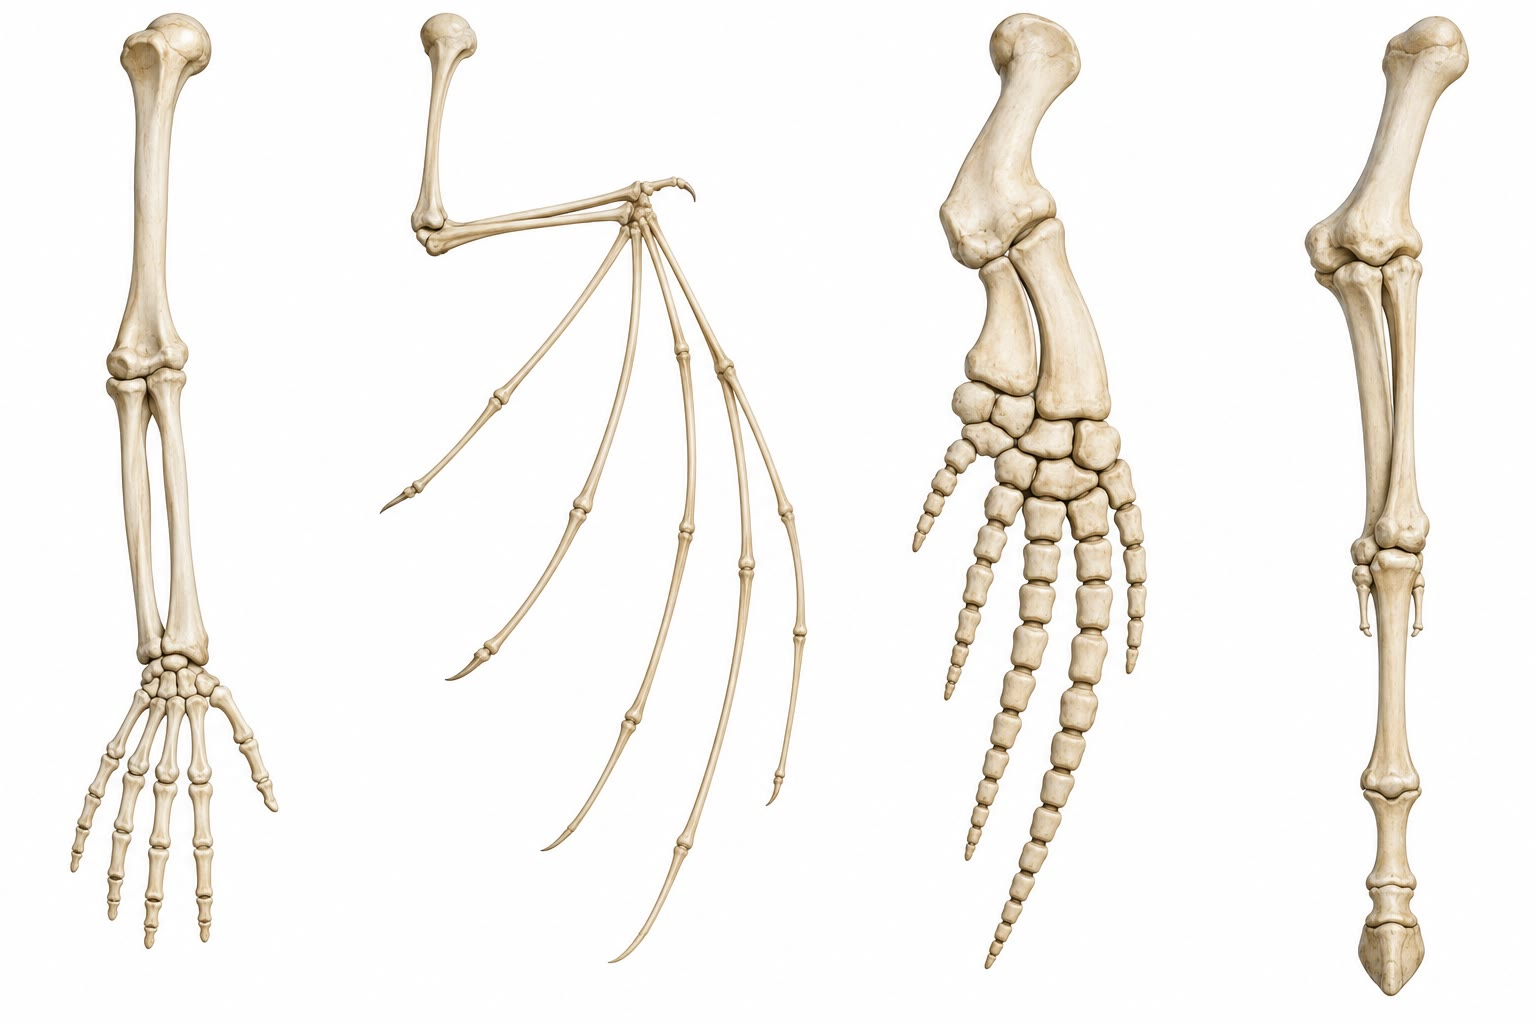
\includegraphics[width=0.44\linewidth]{images/book4/ai/b4-24-homologous-forelimbs.jpg}\hspace{0.04\linewidth}
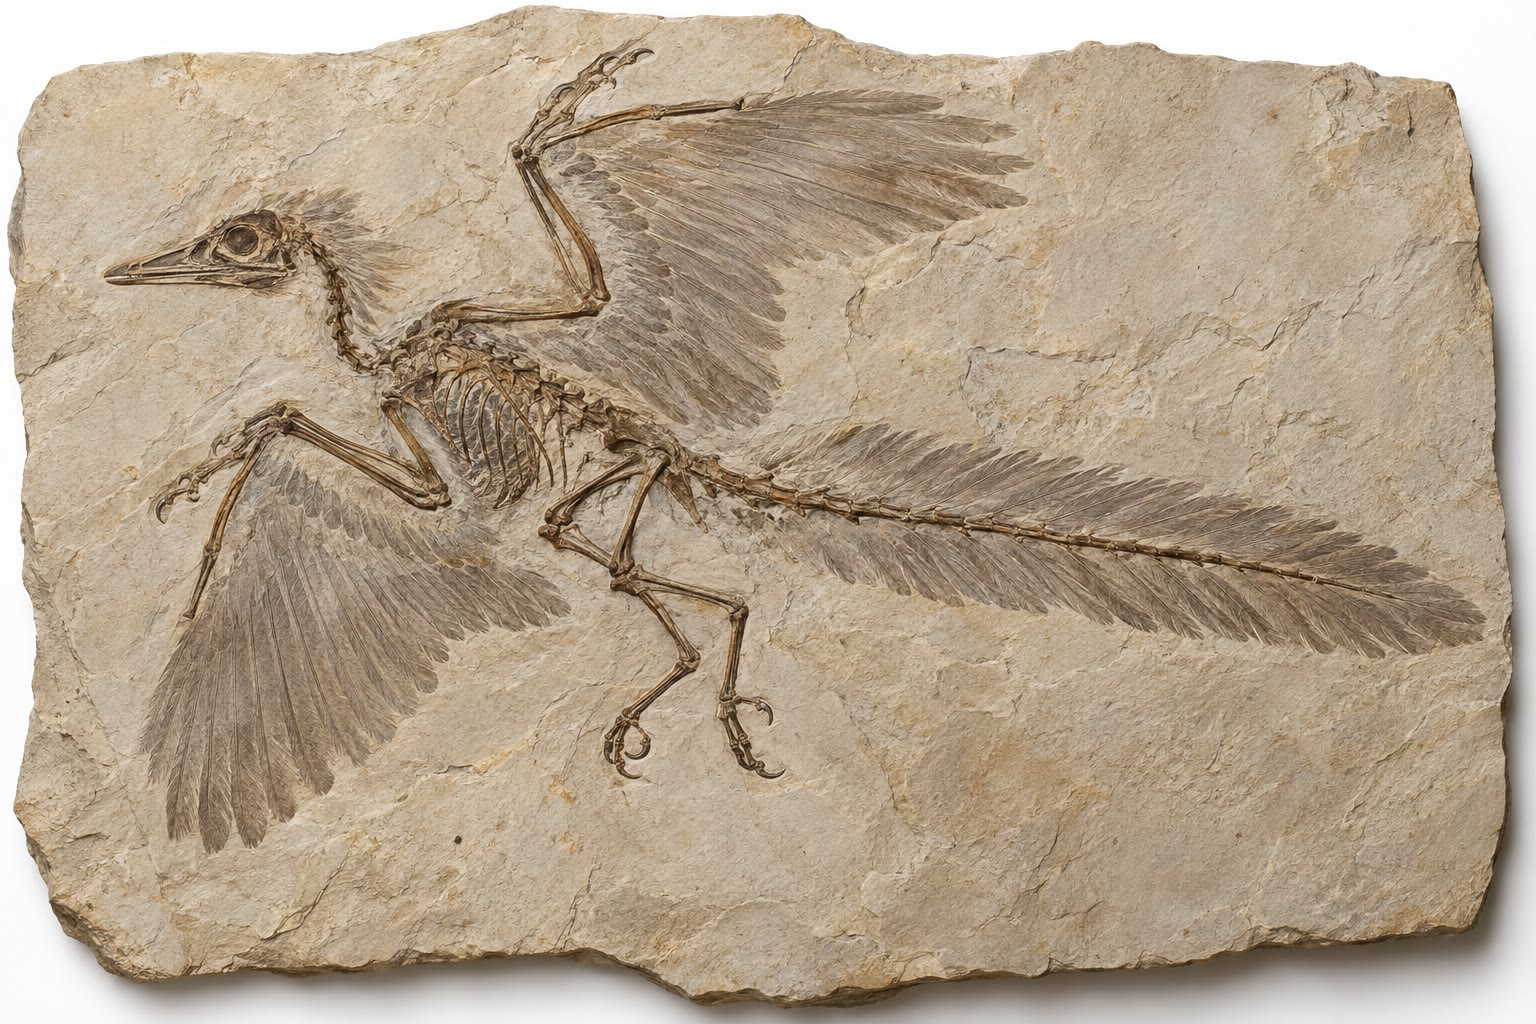
\includegraphics[width=0.44\linewidth]{images/book4/ai/b4-24-archaeopteryx.jpg}

{\small \omterm{def:b2:phylogenetic-trees:tree}{التماثل} وسجله. إلى اليسار: العظام نفسها --- العضد،
والكعبرة والزند، والرسغ، والأصابع الخمس --- في ذراع وجناح وزعنفة
ورجل. وإلى اليمين: \emph{Archaeopteryx}، بأسنانه وأصابعه
المخلبية وذيله العظمي الطويل كديناصور صغير وبريش
طائر.}
\end{omfigure}

\section{بناء الأشجار من الصفات}

\begin{method}[الاقتصاد]\label{meth:b2:phylogenetic-trees:parsimony}
\index{اقتصاد}\index{مجموعة خارجية}\index{بوتستراب}
رمّز الصفات (حالات شكلية أو مواضع متوالية مصطفّة)
لكل وحدة تصنيفية. ثم عُدّ، لكل شجرة ممكنة، أصغر
عدد من تغيرات الصفات يلزم لتفسير المعطيات
عليها؛ فالشجرة الأكثر اقتصادًا تحتاج أقلها. وجذّر الشجرة \emph{\omterm{meth:b2:phylogenetic-trees:parsimony}{بمجموعة
خارجية}}، وهي وحدة تصنيفية يُعلم وقوعها خارج المجموعة المدروسة.
ولمّا كان عدد الأشجار غير المجذّرة عند $n$ وحدة هو $1\cdot 3\cdot
5\cdots(2n - 5)$ --- أي ثلاثة لأربع وحدات، و$2\times 10^{6}$ لعشر،
و$10^{20}$ لعشرين --- كان البحث شاملًا في المجموعات الصغيرة
فقط واستدلاليًا فيما وراءها. وتُقاس الثقة
\emph{بالبوتستراب}: أعد أخذ عينة من الصفات مع الإعادة
ألف مرة، وأعد بناء الشجرة في كل مرة، وسجّل كم مرة يتكرر
كل \omterm{def:b2:phylogenetic-trees:tree}{فرع حيوي}؛ فالفرع الموجود في \qty{95}{\%} من العينات
مدعوم جيدًا، والموجود في نصفها ليس كذلك.
\end{method}

\begin{example}[أربع وحدات وخمسة مواقع]\label{ex:b2:phylogenetic-trees:parsimony}
المتواليات $A = \mathrm{AAGCT}$ و$B = \mathrm{AAGCC}$ و$C =
\mathrm{GGACT}$ و$D = \mathrm{GGATC}$. فعلى الشجرة $((A,B),(C,D))$
تتغير المواقع 1 و2 و3 مرة واحدة كل منها (على الفرع الداخلي)، ويتغير الموقع 4
مرة واحدة ($\mathrm{C}\to\mathrm{T}$ في $D$) والموقع 5 مرتين
($\mathrm{T}\to\mathrm{C}$ في $B$ وفي $D$): أي ست خطوات. وعلى
$((A,C),(B,D))$ تحتاج المواقع 1--3 تغيرين لكل منها، والموقعان 4 و5
تغيرًا واحدًا لكل منهما: أي ثماني. وعلى $((A,D),(B,C))$: تسع. فالشجرة الأولى هي الأكثر
اقتصادًا، بخطوتين؛ والمواقع الثلاثة التي تدعمها هي
صفاتها المشتقة المشتركة، والموقع 5 \omterm{def:b2:phylogenetic-trees:tree}{تشابه عارض} عليها --- أي التغير نفسه
واقعًا مرتين، وهو أمر واقع في كل مجموعة معطيات حقيقية.
\end{example}

\begin{omfigure}
\begin{tikzpicture}[every node/.style={font=\scriptsize}, line width=0.8pt]
  \foreach \x/\a/\b/\c/\d/\steps/\lab in {0/A/B/C/D/6/{$((A,B),(C,D))$ --- 6 خطوات}, 4.6/A/C/B/D/8/{$((A,C),(B,D))$ --- 8 خطوات}, 9.2/A/D/B/C/9/{$((A,D),(B,C))$ --- 9 خطوات}} {
    \begin{scope}[xshift=\x cm]
      \draw (0,1.6) node[left] {\a} -- (0.8,1.1) -- (0,0.6) node[left] {\b};
      \draw (0.8,1.1) -- (2.0,1.1);
      \draw (2.8,1.6) node[right] {\c} -- (2.0,1.1) -- (2.8,0.6) node[right] {\d};
      \node[anchor=north] at (1.4,0.2) {\lab};
    \end{scope}
  }
  \node[anchor=north] at (5.9,-0.6) {\begin{tabular}{l@{\ }ccccc} الموقع & 1 & 2 & 3 & 4 & 5 \\ \hline $A$ & A & A & G & C & T \\ $B$ & A & A & G & C & C \\ $C$ & G & G & A & C & T \\ $D$ & G & G & A & T & C \end{tabular}};
\end{tikzpicture}

{\small الأشجار الثلاث غير المجذّرة لأربع وحدات، مرمَّزة في مقابل
الاصطفاف ذي المواقع الخمسة تحتها. فالمواقع 1--3 تتغير مرة واحدة على الشجرة
الأولى ومرتين على الأخريين؛ والموقع 4 يتغير في وحدة واحدة فقط
فلا يستطيع الحسم، أما الموقع 5 فيجمع $A$ مع $C$ ومن ثم يحبّذ
الشجرة الثالثة عليهما.}
\end{omfigure}

\section{بناء الأشجار من المسافات}

\begin{method}[التعنقد بالمسافة: UPGMA]\label{meth:b2:phylogenetic-trees:upgma}
\index{UPGMA}\index{ضم الجيران}\index{مصفوفة مسافات}
من المسافات الثنائية بين $n$ وحدة تصنيفية (أي الفروق في الموقع،
مصححة كما يأتي)، صِلْ أقرب زوج في عنقود يوضع عند
عقدة ارتفاعها نصف مسافتهما؛ واستبدل بالزوج
العنقودَ، ومسافته إلى كل وحدة أخرى متوسط مسافات
عضويه؛ وكرر حتى يبقى عنقود واحد. والنتيجة
شجرة مجذّرة كل أطرافها على الارتفاع نفسه --- فهي تفترض
معدل تغير ثابتًا على كل فرع، أي \omterm{thm:b2:phylogenetic-trees:clock}{ساعة جزيئية}. وحين
تختلف المعدلات بين السلالات، تجمع الطريقة السلالات السريعة التطور
معًا مهما كان تاريخها؛ أما \emph{\omterm{meth:b2:phylogenetic-trees:upgma}{ضم الجيران}}،
الذي يصل في كل خطوة الزوجَ الذي يقصّر اتحاده الشجرةَ
كلها أكثر، فلا يفترض ساعة وهو الطريقة السريعة المعيارية
لمجموعات المعطيات الكبيرة.
\end{method}

\begin{example}[UPGMA]\label{ex:b2:phylogenetic-trees:upgma}
المسافات (بالفروق في كل مئة موقع): $AB = 4$ و$AC = 8$
و$AD = 10$ و$BC = 8$ و$BD = 10$ و$CD = 6$. صِلْ $A$ و$B$ عند الارتفاع 2؛
ثم $d(AB, C) = 8$ و$d(AB, D) = 10$ و$d(C,D) = 6$: فصِلْ $C$ و$D$ عند
الارتفاع 3؛ وأخيرًا $d(AB, CD) = (8 + 10 + 8 + 10)/4 = 9$: فصِلْ
العنقودين عند الارتفاع $4.5$. فالشجرة هي $((A,B),(C,D))$، وإذا كان
المعدل $10^{-9}$ استبدال في الموقع في السنة كان عمر الجذر
$0.045/10^{-9} = 45$ مليون سنة.
\end{example}

\begin{omfigure}
\begin{tikzpicture}[every node/.style={font=\scriptsize}, line width=0.8pt, x=1.1cm]
  \draw[->] (0,-0.4) -- (5,-0.4); \foreach \h in {0,1,2,3,4} \draw (\h,-0.5) -- (\h,-0.3) node[below=4pt] {\h};
  \node[anchor=north] at (2.5,-0.9) {ارتفاع العقدة (الفروق في كل مئة موقع)};
  % A,B join at 2, C,D at 3, root at 4.5 ; draw as rooted tree, root on the right
  \draw (0,3.0) node[left] {$A$} -- (2,3.0) -- (2,2.4) -- (0,2.4) node[left] {$B$};
  \draw (0,1.2) node[left] {$C$} -- (3,1.2) -- (3,0.4) -- (0,0.4) node[left] {$D$};
  \draw (2,2.7) -- (4.5,2.7) -- (4.5,0.8) -- (3,0.8);
  \fill (2,2.7) circle (1.5pt); \fill (3,0.8) circle (1.5pt); \fill (4.5,1.75) circle (1.5pt);
  \node[anchor=west] at (4.6,1.75) {الجذر، 4.5};
  \node[anchor=south west] at (2.05,3.05) {2};
  \node[anchor=south west] at (3.05,1.25) {3};
  \node[anchor=west, align=left] at (6.2,2.4) {\begin{tabular}{c|ccc} & $B$ & $C$ & $D$ \\ \hline $A$ & 4 & 8 & 10 \\ $B$ & & 8 & 10 \\ $C$ & & & 6 \end{tabular}};
  \node[anchor=west, align=left] at (6.2,0.7) {بعد وصل $AB$:\\ $d(AB,C) = 8$، $d(AB,D) = 10$\\ وبعد وصل $CD$: $d(AB,CD) = 9$};
\end{tikzpicture}

{\small طريقة UPGMA على أربع وحدات. كل عقدة تجلس عند نصف المسافة
بين العنقودين اللذين تصلهما؛ وكل طرف ينتهي عند الارتفاع صفر، كما
تقتضي الساعة.}
\end{omfigure}

\section{الساعة الجزيئية}

\begin{theorem}[الاستبدالات عمليةً بواسونية، وتصحيح الإصابات المتعددة]\label{thm:b2:phylogenetic-trees:clock}
\index{ساعة جزيئية}\index{تصحيح جوكس--كانتور}\index{إشباع}
إذا وقعت الاستبدالات في موقع بمعدل ثابت $k$ في السنة،
مستقلةً عبر المواقع، كان عدد ما يتراكم منها على امتداد
سلالة في زمن $t$ بواسونيًا بمتوسط $kt$، وكان العدد المنتظر
الفاصل بين سلالتين تباعدتا منذ $t$ سنة
\[
d = 2kt
\]
استبدالًا في الموقع --- وهي \emph{\omterm{thm:b2:phylogenetic-trees:clock}{الساعة الجزيئية}}. والنسبة الملحوظة
$p$ للمواقع المختلفة أصغر من $d$، لأن الموقع
المصاب مرتين قد يعود إلى أساسه الأصلي أو يتطابق بالمصادفة؛
وبأربعة أسس تتغير بمعدلات متساوية،
\[
p = \tfrac{3}{4}\bigl(1 - e^{-4d/3}\bigr), \qquad
d = -\tfrac{3}{4}\ln\bigl(1 - \tfrac{4}{3}p\bigr),
\]
وهو تصحيح \emph{جوكس--كانتور}. وإذ يكبر $d$ يتشبع $p$ عند
$3/4$ --- فمتواليتان عشوائيتان تتفقان في ربع مواقعهما
--- وفيما وراء $p \approx 0.5$ يضخّم التصحيح كل
خطأ معاينة: فالمورّثة التي تغيرت ذلك المقدار كفّت عن
حفظ الوقت. والمورّثات البطيئة (RNA الريباسي والهستونات) تؤرخ الفروع
العميقة، والسريعة (DNA المتقدري والقطع الداخلية) تؤرخ الحديثة.
\end{theorem}
\begin{proof}
ليكن $q(t)$ احتمال أن يبقى الموقع حاملًا أساسه
الأصلي بعد زمن $t$. فهو يُفقد بمعدل $k$ ويُستعاد،
من أي من الأسس الثلاثة الأخرى، بمعدل $k/3$:
$\mathrm{d}q/\mathrm{d}t = -kq + \tfrac{k}{3}(1 - q) = \tfrac{k}{3} -
\tfrac{4k}{3}q$، وحله عند $q(0) = 1$ هو $q = \tfrac14 +
\tfrac34 e^{-4kt/3}$. وسلالتان يفصلهما زمن كلي $2t$ ---
وهو، بالتناظر، كسلالة واحدة تتطور مدة $2t$ --- تتفقان عند
موقع باحتمال $\tfrac14 + \tfrac34 e^{-4d/3}$ حيث $d =
2kt$، فيكون $p = 1 - q = \tfrac34(1 - e^{-4d/3})$؛ وبقلبها نحصل على
التصحيح. والعدّ البواسوني يتبع من أحداث ثابتة مستقلة،
كما في فيزياء التفكك الإشعاعي، وانحرافه
المعياري $\sqrt{kt}$ يقرر دقة أي تأريخ: فمورّثة من $L$
موقع فيها $dL$ استبدالًا ملحوظًا تؤرخ تباعدًا بدقة
نسبية قدرها نحو $1/\sqrt{dL}$.
\end{proof}
\begin{proof}[شواهد]
وجد زوكركاندل وبولنغ (1965) أن الفروق بين
خضابات دم الحصان والإنسان والبقرة وغيرها تتناسب مع
أعمار انفصالاتها الأحفورية، فاقترحا الساعة. وبنى فيتش
ومارغولياش (1967) شجرة لعشرين نوعًا من السيتوكروم
$c$ وحده واستعادا، من بروتين واحد، التجمعات
الكلاسيكية للفقاريات والحشرات والفطريات. وكان الاختبار الحاسم
للطريقة هو \omterm{def:b2:phylogenetic-trees:tree}{الشجرة النشوئية} التجريبية التي أجراها هيليس وزملاؤه (1992):
إذ مرّروا العاثية T7 عبر سلسلة متفرعة معلومة
من ثماني سلالات تحت مطفّر، وتسلسلوا النواتج، وأعطوا
المتواليات لطرائق بناء الأشجار على العمياء --- فاستعادت الشجرةَ الحقيقية
طرائقُ الاقتصاد والمسافة والأرجحية جميعًا،
وأعاد الاقتصاد بناء المتواليات السلفية بدقة تفوق
\qty{98}{\%}.
\end{proof}

\begin{omfigure}
\begin{tikzpicture}
\begin{axis}[
  width=0.7\linewidth, height=5.4cm,
  axis x line=bottom, axis y line=left,
  xmin=0, xmax=2.5, ymin=0, ymax=1.05,
  xlabel={الاستبدالات الحقيقية في الموقع، $d$}, ylabel={الفروق الملحوظة، $p$},
  xlabel style={font=\small, at={(axis description cs:0.5,-0.13)}, anchor=north},
  ylabel style={font=\small},
  tick label style={font=\small}, ytick={0,0.25,0.5,0.75,1},
  legend style={font=\scriptsize, at={(0.97,0.35)}, anchor=east, draw=none},
  clip=false,
]
\addplot[very thick, omDef, domain=0:2.5, samples=80] {0.75*(1-exp(-4*x/3))};
\addlegendentry{$p = \tfrac34(1 - e^{-4d/3})$}
\addplot[thick, gray, dashed, domain=0:1.05, samples=2] {x};
\addlegendentry{$p = d$: بلا إصابات متعددة}
\draw[dotted, gray] (axis cs:0,0.75) -- (axis cs:2.5,0.75); \node[font=\scriptsize, anchor=south east] at (axis cs:2.5,0.75) {الإشباع، $p = 3/4$};
\draw[<->, omThm, thick] (axis cs:0.383,0.30) -- (axis cs:0.383,0.383); \node[font=\scriptsize, omThm, anchor=west] at (axis cs:0.5,0.22) {$p = 0.30$ تعني $d = 0.38$};
\end{axis}
\end{tikzpicture}

{\small الإصابات المتعددة. كسر المواقع المختلفة الملحوظ
يرتفع مع العدد الحقيقي للاستبدالات ثم يتشبع؛ و$p$
الخام يقلل من شأن كل مسافة ويضغط الفروع
العميقة في الشجرة.}
\end{omfigure}

\begin{proposition}[مصائد الساعة والأشجار]\label{prop:b2:phylogenetic-trees:pitfalls}
\index{انجذاب الفروع الطويلة}\index{اختلاف المعدلات}\index{الفرز الناقص للسلالات}\index{أرجحية (نشوئية)}
الساعة ثابتة على وجه التقريب فقط: فالمعدلات تختلف بين
المورّثات بمئة ضعف (بحسب الوظيفة --- فالهستون H4 تغير
بقيتين في مليار سنة، وببتيدات الفبرين تتغير كل بضعة
ملايين)، وبين المواقع داخل المورّثة الواحدة (فالمواضع الثالثة في الرمزات،
والقطع الداخلية والعُرى أسرعها تغيرًا)، وبين السلالات (فالقوارض
تدق أسرع من الرئيسيات، بأجيالها الأقصر
واستقلابها الأعلى). ولذلك تحتاج كل ساعة
\emph{معايرة} بأحفورة أو بحدث جيولوجي مؤرخ،
وتحمل التواريخ الخطأ البواسوني المذكور وخطأ المعايرة نفسها.
وللأشجار مصائدها الخاصة. \emph{\omterm{prop:b2:phylogenetic-trees:pitfalls}{فانجذاب الفروع الطويلة}}: سلالتان
تغيرت كل منهما كثيرًا تتفقان في مواقع كثيرة
بالمصادفة، فيصلهما الاقتصاد مهما كان تاريخهما --- وعلاجه
معاينة أكثف لكسر الفروع وطريقة
تنمذج المعدلات. \emph{والتقارب} ينتج صفات مشتقة مشتركة كاذبة.
\emph{\omterm{prop:b2:phylogenetic-trees:pitfalls}{والفرز الناقص للسلالات}}: شجرة المورّثة ليست بالضرورة
شجرة النوع حين تتلاحق الانتواعات بسرعة، لأن
تعدد الأشكال السلفي يُفرز فرزًا مختلفًا في كل سليل
--- ولذلك تُبنى شجرة الأنواع من مورّثات كثيرة لا من واحدة. وفي
بدائيات النوى، حيث تتحرك المورّثات جانبيًا
(\cref{ch:b2:genome-diversification})، تروي مورّثات مختلفة
قصصًا مختلفة ويكون التاريخ شبكة تجري فيها شجرة المورّثات
الريباسية. والممارسة الحديثة تستبدل \emph{بالأرجحية} الاقتصادَ
والمسافة: فبمعطى نموذج للاستبدال (أي معدلات كل
تغير، وتباينها بين المواقع)، احسب
احتمال المتواليات الملحوظة على كل شجرة بأطوال فروعها،
واختر الشجرة التي تجعل المعطيات أرجح ما تكون؛
وصورتها البايزية تعطي احتمالًا لكل \omterm{def:b2:phylogenetic-trees:tree}{فرع حيوي} مباشرةً.
ومجلد السنة الثالثة يعطي الطرائق؛ ويكفي هنا أن نعلم أن
كل شجرة فرضية بدعم مقيس، لا واقعة.
\end{proposition}
\begin{proof}[شواهد]
قارن ووز وفوكس (1977) RNA الريباسي للوحيدة الصغيرة عبر
بدائيات النوى فوجدا المولّدات للميثان بعيدة عن البكتيريا
بعد أي منهما عن حقيقيات النوى: أي المجالات الثلاثة، وقد أكدتها منذ ذلك الحين كل
مورّثة في آلة الاستنساخ والترجمة، وهي
خفية على الشكل. والأشجار الريباسية نفسها، إذا قُرئت ساذجةً،
وضعت البوغيات الدقيقة السريعة التطور عند قاعدة
حقيقيات النوى؛ لكن مورّثات أبطأ معدلًا، ونماذج تسمح بتباين
المعدلات، نقلتها إلى الفطريات حيث تنتمي --- وهي
حالة مدرسية لانجذاب فروع طويلة كُشف وعولج.
\end{proof}

\begin{omfigure}
\begin{tikzpicture}[every node/.style={font=\scriptsize}, line width=0.8pt]
  \node[anchor=south] at (1.5,2.6) {الشجرة الحقيقية};
  \draw (0,2.2) node[left] {$A$} -- (0.8,1.6) -- (0,1.0) node[left] {$B$};
  \draw (0.8,1.6) -- (1.6,1.6);
  \draw[very thick, omThm] (1.6,1.6) -- (3.4,2.4) node[right] {$C$ (سريع)};
  \draw[very thick, omThm] (0.8,1.6) -- (0.8,0.2) -- (2.6,0.2) node[right] {$D$ (سريع)};
  \draw (1.6,1.6) -- (2.4,1.0) node[right] {$E$};
  \begin{scope}[xshift=7cm]
    \node[anchor=south] at (1.5,2.6) {الشجرة التي يجدها الاقتصاد};
    \draw (0,2.2) node[left] {$A$} -- (0.8,1.6) -- (0,1.0) node[left] {$B$};
    \draw (0.8,1.6) -- (1.6,1.6);
    \draw (1.6,1.6) -- (2.4,1.9) node[right] {$E$};
    \draw[very thick, omThm] (1.6,1.6) -- (2.2,1.0) -- (3.4,1.3) node[right] {$C$};
    \draw[very thick, omThm] (2.2,1.0) -- (3.0,0.2) node[right] {$D$};
  \end{scope}
  \node[align=center, text width=7cm] at (5.6,-1.1) {تغيّر $C$ و$D$ كل منهما في مواقع كثيرة؛ وهما يتفقان الآن بالمصادفة في ربعها، وهو أكثر مما تصلهما به أي صفة مشتقة مشتركة حقيقية بأقربائهما الحقيقيين};
\end{tikzpicture}

{\small \omterm{prop:b2:phylogenetic-trees:pitfalls}{انجذاب الفروع الطويلة}. السلالتان الأسرع تطورًا
يصلهما ما تنتجه تغيراتها الكثيرة من تطابقات
بالمصادفة، فيجعلهما الاقتصاد شقيقتين.}
\end{omfigure}

\begin{example}[التأريخ بأحفورة]\label{ex:b2:phylogenetic-trees:dating}
مورّثة من \num{1000} موقع تختلف في \qty{10}{\%} منها بين
البقرة والحوت، وقد وضعت الأحافير سلفهما المشترك عند 60 مليون
سنة. وبالتصحيح يكون $d = -0.75\ln(1 - 0.133) = 0.107$؛ ويكون المعدل $k
= d/2t = 0.107/(1.2\times 10^{8}) = 9\times 10^{-10}$ في الموقع في
السنة. وتختلف المورّثة نفسها في \qty{6}{\%} بين الحوت وفرس النهر:
فيكون $d = 0.0625$ و$t = d/2k = 35$ مليون سنة، مع نحو $\pm
\qty{13}{\%}$ من العدّ البواسوني البالغ 62 استبدالًا ومع
لايقين آخر من تاريخ الأحفورة. أما النتيجة الجزيئية
القائلة إن الحيتان أقرب أقرباء فرس النهر الأحياء، وقد نُيلت
هكذا في التسعينيات ضد كل شجرة تشريحية، فقد أكدها
اكتشاف حيتان مبكرة لها عظم الكاحل الشبيه بفرس النهر
المتنبأ به --- فالساعة لا تؤرخ فحسب؛ بل تتنبأ بما
ينبغي أن تحمله الصخور.
\end{example}

\section{تمارين}

\begin{exercise}[$\star$]\label{exo:b2:phylogenetic-trees:1}
عرّف \omterm{def:b2:phylogenetic-trees:tree}{التماثل} \omterm{def:b2:phylogenetic-trees:tree}{والتشابه العارض} \omterm{def:b2:phylogenetic-trees:tree}{والصفة المشتقة المشتركة}، مع مثال واحد
لكل منها بين أطراف الفقاريات وأجنحتها وعيونها.
\end{exercise}

\begin{exercise}[$\star$]\label{exo:b2:phylogenetic-trees:2}
صنّف ما يلي أحادي العرق أو شبه عرقي أو متعدد العرق: الطيور؛
والزواحف (دون الطيور)؛ والأسماك (دون رباعيات الأطراف)؛ والفقاريات
الطائرة؛ والثدييات؛ وبدائيات النوى.
\end{exercise}

\begin{exercise}[$\star$]\label{exo:b2:phylogenetic-trees:3}
على الشجرة $(\text{الثدييات},(\text{السلاحف},(\text{السحالي},
(\text{التماسيح},\text{الطيور}))))$، سمِّ المجموعة الشقيقة
للطيور، والمجموعة الشقيقة للثدييات، وأصغر \omterm{def:b2:phylogenetic-trees:tree}{فرع حيوي}
يضم السحالي والطيور. وهل يغيّر تبديل موضعي
التماسيح والطيور الشجرةَ؟
\end{exercise}

\begin{exercise}[$\star$]\label{exo:b2:phylogenetic-trees:4}
كم شجرة غير مجذّرة توجد عند 4 و6 و10 وحدات تصنيفية؟ وكم شجرة
مجذّرة لأربع (إذ يمكن تجذير كل شجرة غير مجذّرة على أي من
فروعها)؟
\end{exercise}

\begin{exercise}[$\star\star$]\label{exo:b2:phylogenetic-trees:5}
المتواليات $A = \mathrm{CCTAG}$ و$B = \mathrm{CCTGG}$ و$C =
\mathrm{TTCAG}$ و$D = \mathrm{TTCGA}$. عُدّ الخطوات على كل من
الأشجار الثلاث غير المجذّرة وأعطِ الأكثر اقتصادًا. وأي
المواقع متشابهة عرضًا عليها؟
\end{exercise}

\begin{exercise}[$\star\star$]\label{exo:b2:phylogenetic-trees:6}
المسافات (في كل مئة موقع): $AB = 6$ و$AC = 14$ و$AD = 16$
و$BC = 14$ و$BD = 16$ و$CD = 10$. ابنِ شجرة UPGMA بارتفاعات
عقدها.
\end{exercise}

\begin{exercise}[$\star\star$]\label{exo:b2:phylogenetic-trees:7}
صحّح $p = 0.05$ و$0.30$ و$0.60$ للإصابات المتعددة. ولماذا كانت
القيمة الثالثة شبه عديمة الفائدة؟
\end{exercise}

\begin{exercise}[$\star\star$]\label{exo:b2:phylogenetic-trees:8}
مورّثة تتطور بمعدل $10^{-9}$ استبدال في الموقع في السنة. ونوعان
يختلفان بمقدار $d = 0.02$: فمتى انفصلا؟ وأي $p$ كنت
ستلاحظ بين نوعين انفصلا قبل 500 مليون سنة،
وبماذا يوحي ذلك لتأريخ الانفصالات العميقة بهذه المورّثة؟
\end{exercise}

\begin{exercise}[$\star\star$]\label{exo:b2:phylogenetic-trees:9}
يظهر \omterm{def:b2:phylogenetic-trees:tree}{فرع حيوي} في \qty{52}{\%} من \num{1000} عينة بوتستراب؛
ويظهر آخر في \qty{99}{\%}. فسّر الاثنين. وماذا كنت فاعلًا حيال
الأول؟
\end{exercise}

\begin{exercise}[$\star\star\star$]\label{exo:b2:phylogenetic-trees:10}
فسّر \omterm{prop:b2:phylogenetic-trees:pitfalls}{انجذاب الفروع الطويلة} بحجة الربع بالمصادفة
وقل لماذا تنفع إضافة وحدات تصنيفية تكسر الفروع الطويلة.
\end{exercise}

\begin{exercise}[$\star\star\star$]\label{exo:b2:phylogenetic-trees:11}
يختلف DNA المتقدري للإنسان والشمبانزي في \qty{9}{\%} من
المواقع؛ والمعدل المتقدري نحو $2\times 10^{-8}$ في الموقع
في السنة. أرّخ الانفصال، وأعطِ اللايقين البواسوني لمورثوم من
\qty{16000}{} موقع، وسمِّ سببين قد يكون الجواب بسببهما
خاطئًا مع ذلك بعامل اثنين.
\end{exercise}

\begin{exercise}[$\star\star\star$]\label{exo:b2:phylogenetic-trees:12}
«شجرة المورّثة ليست شجرة النوع.» ناقش \omterm{prop:b2:phylogenetic-trees:pitfalls}{بالفرز
الناقص للسلالات} والنقل الأفقي وتضاعف المورّثات، وقل
كيف تُنال شجرة النوع مع ذلك.
\end{exercise}

\section{مسألة: تأريخ الحيتان}

\begin{problem}[{مسألة نهاية الأسبوع --- الحوت وفرس النهر والبقرة والخنزير و
الجمل مسلسَلة لمورّثة واحدة: بناء الشجرة بالاقتصاد وبالمسافة،
ومعايرة الساعة على أحفورة، وتأريخ كل انفصال مع
خطئه البواسوني، ومواجهة الشجرة التشريحية بالشجرة
الجزيئية، وتنتهي إلى زمن تباعد الحوت وفرس النهر ومعدل
استبدال المورّثة}]
\label{pb:b2:phylogenetic-trees:1}
مورّثة من \num{1000} موقع مسلسَلة في الحوت ($W$) وفرس النهر
($H$) والبقرة ($C$) والخنزير ($P$) والجمل ($M$، وهو \omterm{meth:b2:phylogenetic-trees:parsimony}{المجموعة الخارجية}). ونسب
المواقع المختلفة الملحوظة: $WH = 0.06$؛ و$WC = HC = 0.10$؛ و$WP =
HP = CP = 0.12$؛ وكل مسافة إلى $M$ هي $0.14$. وتضع الأحافير
الانفصال بين البقرة وخط الحوت وفرس النهر عند 60 مليون سنة.
وستة مواقع مُخبِرة، وحالة الجمل مذكورة أخيرًا:
\begin{center}
\begin{tabular}{l@{\quad}cccccc}
الموقع & 1 & 2 & 3 & 4 & 5 & 6 \\ \hline
$W$ & A & G & T & C & A & G \\
$H$ & A & G & T & C & G & G \\
$C$ & G & A & T & T & G & G \\
$P$ & G & A & C & T & G & A \\
$M$ & G & A & C & T & G & A \\
\end{tabular}
\end{center}

\medskip
\noindent\textbf{الجزء الأول --- الاقتصاد.}
\begin{enumerate}
  \item أي المواقع صفات مشتقة مشتركة للمجموعة $\{W, H\}$؟ وأيها للمجموعة $\{W, H,
        C\}$؟ وأي موقع غير مخبر، وأيها \omterm{def:b2:phylogenetic-trees:tree}{تشابه عارض}
        أو صفة مشتقة منفردة؟
  \item عُدّ خطوات المواقع الستة على الشجرة
        $(M,(P,(C,(W,H))))$.
  \item وعُدّها على شجرة التشريحيين $(M,(P,(W,(C,H))))$،
        وهي تضع فرس النهر مع البقرة بين شفعيات الأصابع وتضع
        الحيتان خارجًا.
  \item أي الشجرتين مفضلة، وبكم خطوة؟ ولماذا كان ذلك
        الهامش ضعيفًا، وما الذي يقويه؟
  \item يعطي البوتستراب \omterm{def:b2:phylogenetic-trees:tree}{الفرع الحيوي} $\{W, H\}$ في \qty{83}{\%} من
        عينات المورّثة كلها. فسّر.
  \item لماذا استُعمل الجمل مجموعةً خارجية، وماذا كان
        سيسوء لو استُعملت سمكة بدلًا منه؟
\end{enumerate}

\medskip
\noindent\textbf{الجزء الثاني --- المسافات.}
\begin{enumerate}[resume]
  \item صحّح قيم $p$ الأربع المتمايزة ($0.06$ و$0.10$ و$0.12$
        و$0.14$) للإصابات المتعددة.
  \item طبّق UPGMA على الوحدات الخمس بالمسافات المصححة و
        أعطِ ارتفاعات العقد.
  \item هل تتفق شجرة المسافات مع شجرة الاقتصاد؟
  \item فسّر لماذا كانت UPGMA ستخفق لو كانت سلالة الحوت قد
        تطورت أسرع مرتين من الأخريات.
  \item احسب عدد الاستبدالات التي تراكمت في المورّثة
        بين الحوت وفرس النهر، وانحرافها البواسوني
        المعياري.
  \item أعطِ الدقة النسبية لتاريخ مبني على ذلك العدّ.
\end{enumerate}

\medskip
\noindent\textbf{الجزء الثالث --- الساعة.}
\begin{enumerate}[resume]
  \item عايِر: من مسافة البقرة إلى (الحوت وفرس النهر) ومن
        أحفورة الستين مليون سنة، احسب المعدل $k$ في الموقع في
        السنة.
  \item أرّخ انفصال الحوت وفرس النهر.
  \item أرّخ انفصال الخنزير وانفصال الجمل.
  \item أعطِ تاريخ الحوت وفرس النهر مع لايقينه البواسوني.
  \item معايرة الأحفورة نفسها غير يقينية بمقدار $\pm 5$
        ملايين سنة. انشر ذلك إلى تاريخ الحوت وفرس النهر.
  \item مورّثة أخرى أسرع تعطي $p = 0.45$ بين الحوت و
        الجمل. صحّحها وعلّق على موثوقيتها لهذا الانفصال.
\end{enumerate}

\medskip
\noindent\textbf{الجزء الرابع --- المواجهة.}
\begin{enumerate}[resume]
  \item تقوم شجرة التشريحيين على عظم الكاحل ذي البكرة
        المزدوجة الذي تشترك فيه البقرة والخنزير وفرس النهر والجمل ولا تشترك فيه
        الحيتان الحية، إذ لا أطراف خلفية لها. فسّر لماذا لا يستطيع
        فقدُ صفة أن يُحسب ضد فرع الحوت وفرس النهر.
  \item وُجدت حيتان أحفورية ذات أطراف خلفية سنة 2001؛ وعظم
        كاحلها ذو بكرة مزدوجة. فماذا يفعل ذلك بالحجة؟
  \item إذا كانت الحيتان داخل شفعيات الأصابع، فهل مجموعة
        «شفعيات الأصابع دون الحيتان» أحادية العرق أو
        شبه عرقية أو متعددة العرق؟
  \item مورّثة ثانية تعطي الشجرة $(M,(P,(H,(W,C))))$. سمِّ سببين
        قد تختلف بهما شجرة المورّثة عن شجرة النوع، وقل
        كيف يُحسم الأمر.
  \item يختلف المورثوم المتقدري للحوت وفرس النهر في
        \qty{25}{\%} من المواقع. صحّحه، وقدّر المعدل
        المتقدري من التاريخ الموجود في السؤال 14.
  \item لماذا كان ذلك المعدل أعلى بكثير من معدل المورّثة النووية؟
  \item اذكر النتيجة: الشجرة، والمعدل النووي $k$، وزمن
        تباعد الحوت وفرس النهر مع لايقينه.
\end{enumerate}
\end{problem}
